\documentclass[a4paper, 12pt]{article}

%%% Работа с русским языком
\usepackage{cmap}					% поиск в PDF
\usepackage{mathtext} 				% русские буквы в формулах
\usepackage[T2A]{fontenc}			% кодировка
\usepackage[utf8]{inputenc}			% кодировка исходного текста
\usepackage[russian]{babel}	% локализация и переносы

%%% Дополнительная работа с математикой
\usepackage{amsmath,amsfonts,amssymb,amsthm,mathtools} % AMS
\usepackage{icomma} % "Умная" запятая: $0,2$ --- число, $0, 2$ --- перечисление

%% Номера формул
%\mathtoolsset{showonlyrefs=true} % Показывать номера только у тех формул, на которые есть \eqref{} в тексте.

%% Шрифты
\usepackage{euscript}	 % Шрифт Евклид
\usepackage{mathrsfs} % Красивый матшрифт

%% Поля
\usepackage[left=2cm,right=2cm,top=2cm,bottom=2cm,bindingoffset=0cm]{geometry}

%% Русские списки
\usepackage{enumitem}
\makeatletter
\AddEnumerateCounter{\asbuk}{\russian@alph}{щ}
\makeatother

%%% Работа с картинками
\usepackage{graphicx}  % Для вставки рисунков
\graphicspath{{images/}{images2/}}  % папки с картинками
\setlength\fboxsep{3pt} % Отступ рамки \fbox{} от рисунка
\setlength\fboxrule{1pt} % Толщина линий рамки \fbox{}
\usepackage{wrapfig} % Обтекание рисунков и таблиц текстом

%%% Работа с таблицами
\usepackage{array,tabularx,tabulary,booktabs} % Дополнительная работа с таблицами
\usepackage{longtable}  % Длинные таблицы
\usepackage{multirow} % Слияние строк в таблице

%% Красная строка
\setlength{\parindent}{2em}

%% Интервалы
\linespread{1}
\usepackage{multirow}

%% TikZ
\usepackage{tikz}
\usetikzlibrary{graphs,graphs.standard}

%% Верхний колонтитул
\usepackage{fancyhdr}
\pagestyle{fancy}

%% Перенос знаков в формулах (по Львовскому)
\newcommand*{\hm}[1]{#1\nobreak\discretionary{}
	{\hbox{$\mathsurround=0pt #1$}}{}}

%% Мои дополнения
\usepackage{float} %Добавляет возможность работы с командой [H] которая улучшает расположение на странице
\usepackage{gensymb} %Красивые градусы
\usepackage{graphicx}               % Импорт изображений
\usepackage{caption} % Пакет для подписей к рисункам, в частности, для работы caption*

% подключаем hyperref (для ссылок внутри  pdf)
\usepackage[unicode, pdftex]{hyperref}

%%% Теоремы
\theoremstyle{plain}                    % Это стиль по умолчанию, его можно не переопределять.
\renewcommand\qedsymbol{$\blacksquare$} % переопределение символа завершения доказательства

\newtheorem{theorem}{Теорема}[section] % Теорема (счетчик по секиям)
\newtheorem{proposition}{Утверждение}[section] % Утверждение (счетчик по секиям)
\newtheorem{definition}{Определение}[section] % Определение (счетчик по секиям)
\newtheorem{corollary}{Следствие}[theorem] % Следстиве (счетчик по теоремам)
\newtheorem{problem}{Задача}[section] % Задача (счетчик по секиям)
\newtheorem*{remark}{Примечание} % Примечание (можно переопределить, как Замечание)
\newtheorem{lemma}{Лемма}[section] % Лемма (счетчик по секиям)

\begin{document}
    \newcommand{\HRule}{\rule{\linewidth}{0.7mm}} % Defines a new command for the horizontal lines, change thickness here
	
	\begin{center}
		\large\textbf{Московский Физико-Технический Институт}\\ % Name of your university/college
		\large\textbf{(государственный университет)}
	
		\vfill
		
		\Large Лабораторная работа по курсу общей физики № *labnum*\\[0.5cm] % Preambule of your document title
		
		
		\HRule
		\\[0.4cm]
		{ \huge \bfseries *name of your labwork*}% Title of your document
		\\[0.4cm] 
		\HRule
		\\[0.5cm]
		
		\ \\
	\textbf{\large Автор:} \\	
	\large *your name* *groupname*\\ % Your name and something more, your group num for example
		\vfill
		\hspace*{-0.8 cm}
\includegraphics[width=100 pt]{frkt_logo}\\ % logo of your  company/university/college
		\large Долгопрудный, 2021 % location and year
	\end{center}

\newpage
\setcounter{page}{2}
\fancyfoot[c]{\thepage}
\fancyhead[L] {Работа № *labnum*} % some information in page header
\fancyhead[R]{}

    Измерим параметры магнитных шариков: $m_1 = 820$ г, $m_2 = 815$ г, $d = 5,9$ мм.\\
    Величину магнитного момента двух одинаковых шариков можно расчитать, зная их массу и определив
    максимальное расстояние $r_{max}$, на котором они удерживают друг друга.

    \begin{equation*}
        P_m = \sqrt{\frac{4 \pi mg r_{max}^4}{6 \mu_0}}
    \end{equation*}

    Перепишем выражение с учетом $\mu_0 = 4 \pi \cdot 10^{-7}$

    \begin{equation*}
        P_m = \sqrt{\frac{mg r_{max}^4}{6} \cdot 10^7}
    \end{equation*}

    В процессе эксперемента получено $r_{max} = 23$ мм.

    \begin{center}
        \fbox{$P_m = 61,84 ~ \text{А} \cdot \text{м}^2$}
    \end{center}

    Горизонтальную составляющую магнитного поля Земли можно найти, используя период крутильных колебаний.

    \begin{equation*}
        T = 2 \pi \sqrt{\frac{J_n}{P_{mn} B_{||}}}
    \end{equation*}
    где $J_n$ -- момент инерции стрелки из $n$ шариков, $P_{mn} = P_m \cdot n$ -- магнитный момент стрелки.
    Момент инерции стрелки приближенно можно считать
    \begin{equation*}
        J_n \approx \frac{1}{3} n^3 m R^2
    \end{equation*} 
    тогда
    \begin{equation*}
        T = 2 \pi \sqrt{\frac{m R^2}{3 P_m B_{||}}} n
    \end{equation*}

    Снимем зависимость и построим график $T(n)$, тогда угловой коэффициент наклона будет равен $k = 2 \pi \sqrt{\frac{m R^2}{3 P_m B_{||}}}$.
    От сюда найдем горизонтальную составляющую магнитного поля Земли: $B_{||} = \frac{m R^2}{3 P_m k^2}$.

    \begin{table}[h!]
        \begin{center}
            \begin{tabular}{|c|c|c|c|c|c|}
                \hline
                $n$ & 11   & 10   & 9   & 8    & 7    \\ \hline
                $T$ & 2,86 & 2,67 & 2,4 & 2,23 & 1,95 \\ \hline
            \end{tabular}
        \end{center}
    \end{table}

    \begin{figure}[h!]
        \centering
        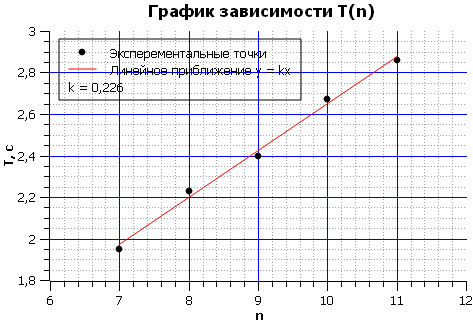
\includegraphics[scale = 1]{T_n_.jpg}
        \caption{}
    \end{figure}

    \begin{center}
        \fbox{$B_{||} = 19,6 $ мкТл}
    \end{center}

    Измерить вертикальную составляющую магнитного поля Земли можно с помощью той же установки, используя уравнение моментов.

    \begin{equation*}
        m g r_{\text{гр}} = n P_m B_{\perp}
    \end{equation*}

    \begin{center}
        \fbox{$B_{\perp} = 47 $ мкТл}
    \end{center}

    Найдем польный модуль магнитного поля Земли на текущей широте.

    \begin{equation*}
        B_0 = \sqrt{B_{||}^2 + B_{\perp}^2} = 44,2 ~ \text{мкТл}
    \end{equation*}

    Исследуем индукцию соленоида. Параметры шайбы: $d = 9$ мм, $h = 4$ мм.

    \begin{table}[h!]
        \begin{center}
            \begin{tabular}{|c|c|c|c|c|c|c|c|c|}
                \hline
                $n$      & 1   & 2   & 3   & 4   & 5   & 6   & 7   & 8   \\ \hline
                $B$, мТл & 232 & 314 & 349 & 355 & 362 & 363 & 364 & 369 \\ \hline
            \end{tabular}
        \end{center}
    \end{table}

    \begin{figure}[h!]
        \centering
        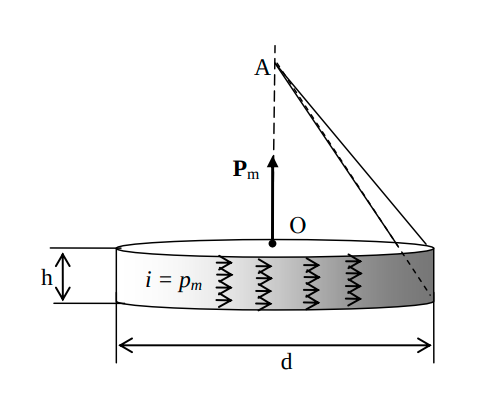
\includegraphics[scale = 0.5]{индукция соленоида.png}
        \caption{}
    \end{figure}

    Магнитное поле в произвольной точке $A$ на оси соленоида расчитывается по формуле

    \begin{equation*}
        B_A = \frac{\mu_0}{4 \pi} 2 \pi i (\cos \alpha - \cos \beta)
    \end{equation*}

    Для точки $O$ на торце соленоида $\cos \beta = 0$, так что для соленоида высотой $h$, радиусом $R$, и магнитным моментом
    $P_m$ поле на торце расчитывается по формуле

    \begin{equation*}
        B(h) = \frac{\mu_0}{2} P_m \frac{h}{\sqrt{R^2 + h^2}}
    \end{equation*}

    Проведем небольшое исследование функции $B(h)$.

    \begin{equation*}
        \lim_{h \rightarrow \infty} \frac{\mu_0}{2} P_m \frac{h}{\sqrt{R^2 + h^2}} = \frac{\mu_0}{2} P_m
    \end{equation*}

    Таким образом, график функции $B(h)$ должен иметь горизонтальную асимптоту $B_0 = \frac{\mu_0}{2} P_m$, что мы и можем
    наблюдать на практике.

    \newpage
    \begin{figure}[h!]
        \centering
        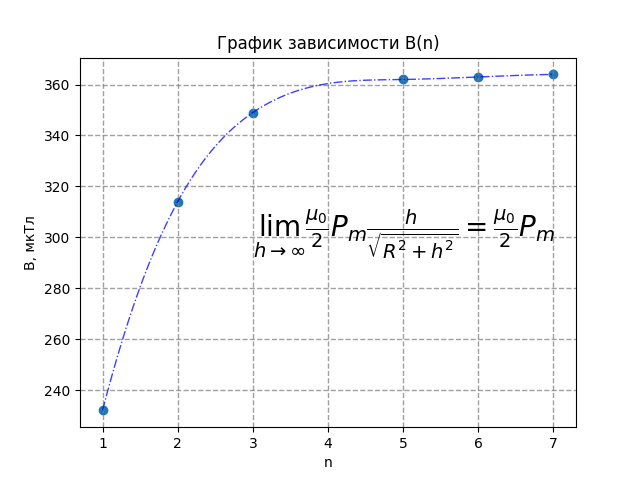
\includegraphics[scale = 1]{solenoid.png}
        \caption{}
    \end{figure}

\end{document}